
\documentclass[12pt,a4paper,oneside]{book}
\usepackage{setspace}
\onehalfspacing
\usepackage[hmargin={2.5cm,2.5cm},vmargin={2.5cm,2.5cm}]{geometry}


\usepackage[english]{babel}
\usepackage[utf8]{inputenc}
\usepackage[T1]{fontenc}


\usepackage[final]{pdfpages} % include pdf files

\usepackage{amsthm}
\usepackage{amsmath}
\usepackage{amsfonts}
\usepackage{tabularx}
\usepackage[nottoc, notlot, notlof, numbib, numindex]{tocbibind}


\usepackage{url}
%\usepackage{geometry}
\usepackage{enumitem}
\usepackage{hyperref}
\usepackage{comment}
\usepackage{listings} 
\usepackage{caption} 
\usepackage{stmaryrd}
\usepackage{fancybox}
\usepackage{makeidx}

\usepackage{eurosym}
\usepackage{multirow}
\usepackage{adjustbox}
\usepackage{charter}
\usepackage{graphicx}

\newcommand{\bp}{\textit{Park~Your~Car }}


\begin{document}
%\maketitle


\begin{titlepage}
\noindent \begin{minipage}{0.83\textwidth}
\noindent \textbf{UNIVERSIDAD CARLOS III DE MADRID}\hfill{}\\
\textbf{Graduate School of Business}\hfill{}\\
\textbf{Master in Management}\hfill{}
\end{minipage}
\begin{minipage}{0.17\textwidth}

\includegraphics[keepaspectratio=true,width=\textwidth]{images/logo_UC3M_universidad_Carlos_III_Madrid.jpg}
\end{minipage}
\begin{center}
\vfill{}\vfill{}\vfill{}
%\begin{center}
{\Huge Business Plan : Park your car}
%\end{center}
{\Huge \par}
\begin{center}{\LARGE Simon \textsc{Picard}}\end{center}{\Huge \par}
%\vfill{}\vfill{}\vfill{}\vfill{}\vfill{}
\vfill{}

\includegraphics[keepaspectratio=true,width=\textwidth-2cm]{images/Seal_of_the_University_of_Carlos_III.jpg}
\vfill{}
\begin{flushleft}{\large \textbf{Supervisor  :}}\\
{\large Prof. Kurt \textsc{Achiel Desender}}
\end{flushleft}{\large\par}
\vfill{}\vfill{}\enlargethispage{2cm}
\textbf{Academic year 2016~-~2017}
\end{center}
\end{titlepage}



\newpage
%\newgeometry{hmargin={3.5cm,1.5cm},vmargin={2.5cm,2.5cm}}
\thispagestyle{empty} 
\null


\tableofcontents

\chapter{Executive Summary}

\chapter{Industry Environment}

\section{Macro Environmental Analysis}

\subsection{Economic}
According to the GDP per capita (PPP), the European Union is the second largest economy in the world. Its total GDP is \euro 16.5 trillions in 2016 , which represents 22.8\% of the global GDP\cite{imfgdp}. The 2008 financial crisis appears to be in the process of recovery, as the economy of 19 of its countries advanced by 0.6 percent over the first three months of the year, as compared to the previous quarter\cite{eurorecov}.\\

Belgium's economy is mainly composed from the service sector, accounting for 74.9\% of its GDP. Belgium also profits from an heavy industrial sector, which is concentrated mainly in northern Flanders, around Brussels and in Liège and Charleroi. The industry sector represents 21.1\% of Belgium's GDP. Finally, the agriculture sector represents less than 1\% of its GDP.\\
With a GDP of \$508.6 billions (PPP, 2016), Belgium ranks itself at the 38th position of the richest country in the world. In 2016, the GDP growth was 1.4\% and the unemployment rate was 8.4\%.\\
With approximately two-third of Belgium's GDP relying on exportation, the country relies heavily on world trade. This high proporation comes from the its skilled, multi-cultural and central population\cite{ciafb}.\\

The economy of Brussels is mainly oriented around the service industry, with 88\% of all jobs being in the service sector. Brussels alone contributes to a fifth of Belgium's GDP. Brussels holds 550 000 jobs and it represent 17.7\% of the country employment. There is 2000 foreign companie offices in the capital.\cite{bxinfo}.\\
Brussels is one of the richest city of the world with a GDP per capita of 67,811 (PPP) in 2016, which ranks it at the 9th position within the raking of the city of the OECD\cite{oecdstat}, Brussels is thus the economic capital of the country. Brussels GDP is boosted by a number of commuter from nearby regions. There is 230 000 employees coming from Flanders and another 130 000 coming from Wallonia working in Brussels. On the other hand, only 16\% of Brussels habitants work outside of the city\cite{euresCom}.\\
Although having apparently a big wealth, Brussels is not the holder of all of it. Indeed, it appears that the proportion of the unemployed resident of Brussels was 20.4\% in December 2013\cite{unemploybx}.

\subsection{Political and legal}

Belgium is a constitutional, popular monarchy and a federal parliamentary democracy. The country is divided in three regions, Wallonia, Flanders and Brussels, which all have regional government.\\
The worldwide governance indicator gives us informations about the political situation of Belgium. The indicators say that the Belgium is a country of low corruption, high government effectiveness, high regulatory quality, high rule of law and high voice and Accountability. Based on those indicators, Belgium lacks political stability and absence of violence/terrosrism with a value in this indicator of 65 in 2015\cite{wbgi}. On the other hand, when compared with other western European countries such as Spain and France, Belgium is valued higher in this field.\\
Part this political stability score can be explained by the language and regional division of the country and subsequently political opinions.\cite{bailo2016political}.\\

The Belgian employment laws are based on the consultation of employee and workers. The lenght of the work is limited to 8 hours per day and 40 hours per week. There is a minimal wage which is valued at \euro 1 501,82 (2015)\cite{eurostatmw}.\\
A new potential law known as "Peteers' Law" is beeing studied, which would make the maximal number of hours that one can work based annualy instead of weekly. This would lead to a potential week of 45 hours.\cite{rtlp} This process shows a trend of work deregulation.\\

As a member of the European Union, Belgium applies the "common customs tariff of the European Union" to goods imported from non-EU countries. Overall, Belgium is open to trade since the country itself relies heavily on it. The trade regulation are decreasing, as one can see from the rise of the European Union, CETA and TAFTA//TTIP. Although those regulation are not currently established, the trend is to facilitate the international trade, specially for Brussels, as the capital of Europe.\\

\subsection{Social}

Belgium as a total population of 11 250 000 (2016) habitants and it is growing at a rate of 0.82\% (2008). 66.3\% of the population is between 15 and 64 years old. Its largest city is Brussels, with a total population of 1 175 173\cite{ciafb}.\\

A current social concern for Belgium is the integration of second and third generation of immigrants. A part of this segment is not integrated to the country whether socioeconomicly of culturally. This phenomenon concern principally groups of young Belgian citizens of Moroccan origin who feel excluded from the society, this is particularly happening in Brussels and Antwerp\cite{sgikc}.\\

As Belgium has 27,3\% of its population younger than 24 years old and its median age is 43.1 years, Belgium has a younger population emerging\cite{ciafb}. It is then relevant to investigate the trends for the millennials and surrounding generation to understand the rises of trends in Belgium. The millenials are higly connected through social media and mobile data. The generation Z is even more. As the first members of the generation Z will turn 21 years old in 2017, their influence will impact the market.\\
This super-connection leads to promotion over social media, platformless shopping and digitalisation. Overall, what is needed is a fast process, with instant notification and picture based description of product\cite{stbe}.



\subsection{Environmental}

Belgium has high density of population which impacts its environment particularly in the major cities of the country. Overall, Belgium is oriented toward an environment friendly approach, being ranked 41 out of 180 in the environment protection index\cite{epi} and Belgium has one the most efficient recycling process. In Flanders, 75 \% of the residential waste produced are reused, recycled or composted\cite{wastemana}.\\

In 2010, a study was conducted about the main mean of transportation of Brussels inhabitant. The result was that, within Brussels, the car was used by 32\% of the population, and for movement to or from Brussels, the car was preferred in 63.6\% of the cases.\cite{mtpd}

\subsection{Technological}
As \bp is designed to be an on demand application present on desktop computer but mainly mobile devices, several technological factors have an impact on the viability of the business.\\

Belgium has a well developed internet infrastructure and rank itself among the most connected country in the world. Belgium has 8.6 millions of internet users, which represent 82.0\% of the population.\cite{intuser} There is 3.6 millions users of fixed broadband and 3.5 millions subscribers of mobile broadband.\cite{intsub} The global coverage of houses is 99.96\% for a 1 Mpbs connection and 91.1\% for a 100 Mbps one.\cite{fixcov} Regarding the mobile coverage, the whole country is covered in 2G connection, almost all the country has access to the 3G network and most urban area have 4G connection.\cite{mobcov}\\

\bp would also rely on cloud technology for the host of the application and the needed computing power. There is lot's of offers of hosting available and it does not rely on the location of the use of the application since Belgium has a fast strong internet coverage.\\

\bp would be part of the on demand economy. This model is based around online platform where independent sellers have an offer for another individual. Classic example of this economy are \textit{Uber} and \textit{eBay}. Recent surveys and data show that this segment is growing and attracting more and more people, not just a young or wealthy population.\cite{odegrow}

\subsection{Conclusion}
This analysis allow us to see that Brussels is a suitable market for \bp.\\
From an economical point view, Brussels' population is wealthy enough to embrace the product. A big part of Brussels' economy comes from the service, which is an industry where there is often mandatory movement by car. Moreover, a lot of employees in Brussels come from outside the city.\\
From the political side, Belgium's government effectiveness is high and there is close to no corruption. Thus \bp would be safe from any sort of blackmail and its legalisation and regulation process would be on time. The business opportunity does not rely on a lot of employment thus the employment law are aligned with it.\\
The Belgium's population is not and old one and it is still growing. Thus the market size is not threatened. The young generation is increasingly tech-savvy which is correlated to the on-demand economy.\\
Environmentally speaking, Belgium's is very conscious. As \bp will reduce non utilised space, improve parking utilisation and prevent potentially new parking lot to emerge, its aim is linked to environmental issues.\\
Finally, Belgium is technologically able to receive the on-demand business. Indeed, the country is very well connected and hosting services are easily available within.

\section{Industry Description and Market Boundaries}
The parking industry is not a straightforward one, it can be free, private or publicly owned.\\
The obvious business offer is the parking offered through the big building designed only for that goal. Those are usually privately owned and are offering spots only in specific locations, usually key locations where there is a lot of demand.\\
Then there is the free parking in the street. When a driver wants to find a spot in the street, he would rely on luck and knowledge of the neighbourhood to find it. In rural or low density area, finding a spot is not a problem as there is low demand. On the other hand, in dense area, the available spots are rather rare because in front of a house there would two spots for ten or more habitants, leading to an offer too small. Free parking are sometime subject to time limit in crowded location, the driver could stay only two hours per example. This process is used to facilitate car turnover.\\
In dense area, the parking are usually subject to charge for non resident of the area. This was developed as a mean to give more liberty to the habitant and incentive people to use another mean of transportation than the car.\cite{nycar} In the same way that for the free parking, the maximum time of stay of non free parking is sometime bounded to a few hours to increase the number of spots available.\cite{bxpay} \\
The other possibility is to buy a parking space in the street, this option is usually linked to a house. A similar process is to rent the space on a monthly basis. Those are approaches that are suitable for long term use, typically when the user lives next to the parking spot and struggle to find free ones.

\subsection{Private Parking Short-Term Rent}
Parking problem arise in dense area, where there is a lot of habitants in the neighbourhood and too few available spots for all of them. A solution to this problem is to charge for parking spots for non resident.\\
First of all, this solution is not perfect, the driver may still struggle to find a spot. Secondly, the parking would not be free for the user if he does not live in the area.\\

On the other hand, there are lot's of empty private parking spaces. Indeed, houses often come with a parking and a parking space driveway but the owner might not have a car, leading to an empty space. More likely, the owner would not use the spot all the time. Per example, if he works in an office, his parking spot would typically be free from 9 am to 5 pm.\\
The \autoref{mapentry} shows how many in street access are present in a selection of street in the west of Brussels. As one can see, the amount of unused space is large.\\


\begin{figure}[h]
\centering
\caption{Access private or public parking\cite{mapentrysrc}}
\label{mapentry}
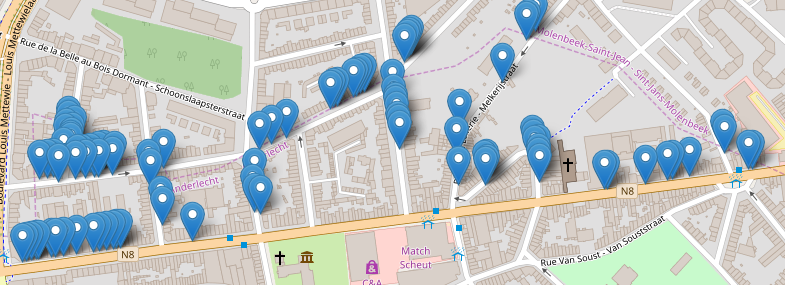
\includegraphics[keepaspectratio=true,width=\textwidth-2cm]{images/casestudyander.png}
\end{figure}

When connecting those two facts, a solution for the parking shortage arise and lead to a non zero sum game. Indeed, if the parking owner rent his space when he does not use it, he would earn money, and the driver would be able to rent the space thus finding a spot easily and he would have to pay anyway to park his car. It is assumed that the driver would have to pay as he would be in a situation where he struggle to find a spot, thus in a dense area, thus a location where the parking is charged.\\

This is ultimately a private parking short-term rent solution.

\subsection{Market Segment}
\bp has to offer its service in dense area. The application will offer its service only in Brussels at first.\\

The choice of focusing only on one region is based on the fact that the application will need network effects to be successful. Thus heavy initial promotion is needed. The goal is to implement the offer successfully in Brussels first and then explore other accurate locations. Offering the private parking short-term rent everywhere, including non dense area, would have bad impact on the image of the application. Indeed, if a user sees that there is no availability in his neighbourhood, he is unlikely to use it again, although there was no availability in his neighbourhood because there was no need.\footnote{survey} \\

Choosing Brussels as a the first city to implement the project is an appropriate choice. Indeed, Brussels is a leading city in Europe. The city is dense. There is 700 000 cars in movement at peak hour for 265 000 available spots.\cite{parkbx} The macro environment presented how Brussels is suitable for \bp. The following map shows the parking rules in Brussels\cite{parkbx} : \\

\begin{figure}[h]
\centering
\caption{Map of Brussels' regulated parking area}
\label{bxmap}
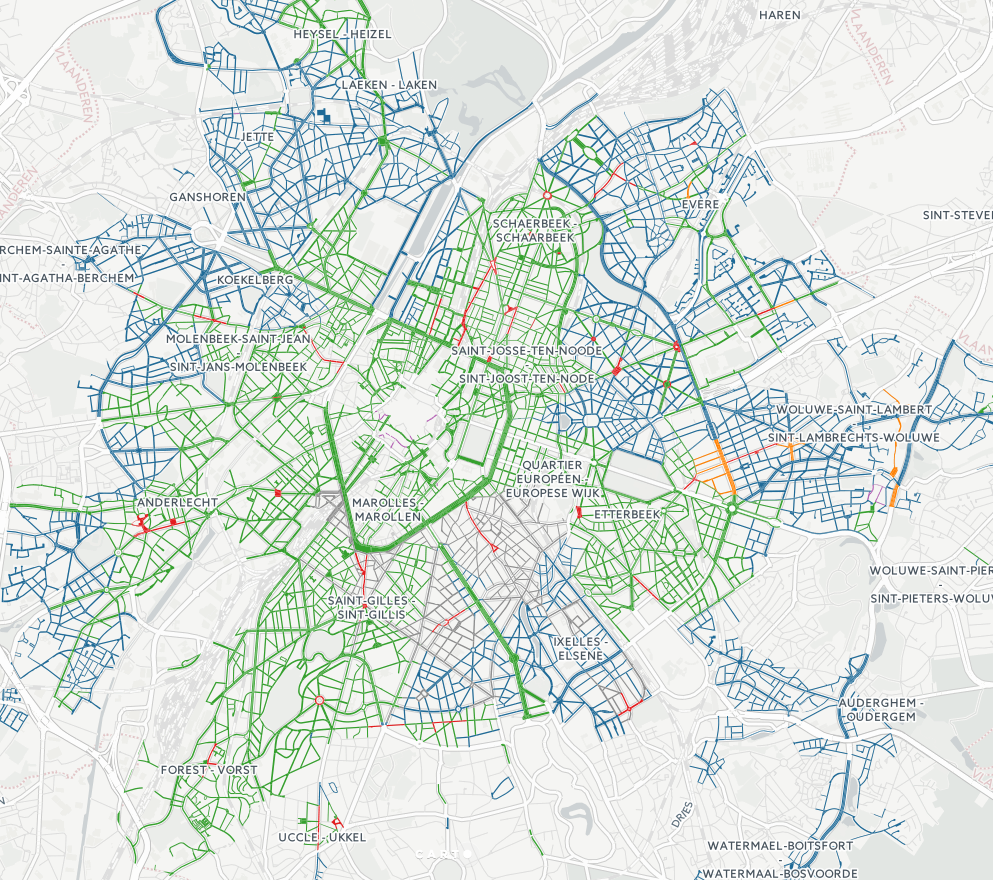
\includegraphics[keepaspectratio=true,width=\textwidth-2cm]{images/bxpark.png}
\end{figure}


The blue area are free but for a length of 2 hours maximum and in the green, grey, orange and red ones, the driver needs to pay to park his car. The \autoref{bxfare} details the price and the maximum time in each zone.\\

\begin{table}[h]
\centering
\caption{Brussels' parking fare}
\label{bxfare}
\begin{tabular}{|l|l|l|l|l|}
\hline
           & Green & Grey & Orange & Red  \\ \hline
Max        & /     & 4:30 & 2:00   & 2:00 \\ \hline
0:30       & 0.50  & 0.50 & 0.50   & 0.50 \\ \hline
1:00       & 1.00  & 1.00 & 1.00   & 2.00 \\ \hline
1:30       & /     & /    & 2.00   & 3.50 \\ \hline
2:00       & 3.00  & 3.00 & 3.00   & 5.00 \\ \hline
3:00       & 4.50  & 5.00 & /      & /    \\ \hline
4:00       & 6.00  & 8.00 & /      & /    \\ \hline
4:30       & /     & 9.50 & /      & /    \\ \hline
Extra hour & 1.50  & /    & /      & /    \\ \hline
\end{tabular}
\end{table}

As a city with an heavily regulated parking policy, Brussels is the ideal candidate for \bp to start its growth.

\subsection{Customer}
The service is based on two types of customer.\\

In the first place, there is the parking space renter. In order to be able to rent a parking spot, one would need to own a parking spot in Brussels. As the parking spot should be free at a recurring schedule in order to rent it consistently, employed people who do not work at home and use the car to go to their work place is an accurate person. One could assume that renting its spot would only attract not wealthy people but renting its spot is also an ecologist act.\footnote{survey} There is also benefit of renting a space if you are a user of the application on the other side as well. Indeed, there would be bonus for space renters.\\

The second type of customer is the one willing to rent a place, the tenant. The people who might fall into that category need to use a car, whether it is owned or leased, in Brussels. They also need to have a smart phone and a mobile internet connection.\\
Whether this group of people will use the service or not is not related to any kind of wealth factor. Indeed, if a driver is looking for a spot and none are available for the period he desires, he cannot pay extra for a free spot, there are none available. If someone on the poor segment of the population is looking for a spot, he will want to find one and pay if needed as he is already in the location and going back home without completing the purpose of the ride is unlikely to be a better option.\\
More than just owning a smart phone, the typical user has to be aware that such technology exists. A person who knows and has used at least once \textit{Uber} would fall into such a category.

\subsection{Suppliers of the Industry}
The supply of the parking industry as a whole are parking spots. For \bp it is precisely private parking spots.\\
The particularity of the business model is that the supplier is also a customer. Indeed, it will be the owner of the parking spot that will have to register itself in the application and enter its parking spot in the system.

\subsection{Competitors}
\subsubsection{Parking Offer Comparison}
\label{poc}
Before analysing \bp 's competitor in its particular business model, it seems appropriate to compare the different parking offer and why \bp 's offer is relevant.\\

The \autoref{parkof} propose a comparison of the different means available to a motorist to park his car. Commercial parking represent big parking lot owned by a private company, private long term parking is a parking owned or rented on a monthly basis, finally private parking short term represent \bp 's offer.

\begin{table}[h]
\centering
\caption{Parking offer comparison}
\label{parkof}
\begin{adjustbox}{center}
\begin{tabular}{l|l|l|l|l|l|}
\cline{2-6}
\multirow{2}{*}{}                           & \multicolumn{2}{c|}{\textbf{Public Parking}}                                                      & \multicolumn{1}{c|}{\multirow{2}{*}{\textbf{\begin{tabular}[c]{@{}c@{}}Commercial\\ Parking\end{tabular}}}} & \multicolumn{1}{c|}{\multirow{2}{*}{\textbf{\begin{tabular}[c]{@{}c@{}}Private Parking\\ Long Term\end{tabular}}}} & \multicolumn{1}{c|}{\multirow{2}{*}{\textbf{\begin{tabular}[c]{@{}c@{}}Private Parking\\ Short Term\end{tabular}}}} \\ \cline{2-3}
                                            & \multicolumn{1}{c|}{\textbf{Free}} & \multicolumn{1}{c|}{\textbf{Regulated}}                      & \multicolumn{1}{c|}{}                                                                                       & \multicolumn{1}{c|}{}                                                                                              & \multicolumn{1}{c|}{}                                                                                               \\ \hline
\multicolumn{1}{|l|}{\textbf{Stay}}         & Very Short                         & Very Short                                                   & \begin{tabular}[c]{@{}l@{}}Short and\\ Long\end{tabular}                                                    & Long                                                                                                               & Short                                                                                                               \\ \hline
\multicolumn{1}{|l|}{\textbf{Price}}        & Free                               & \begin{tabular}[c]{@{}l@{}}Cheap to\\ Expensive\end{tabular} & Expensive                                                                                                   & Moderate                                                                                                           & Cheap                                                                                                               \\ \hline
\multicolumn{1}{|l|}{\textbf{Location}}     & Scarce                             & Frequent                                                     & Scarce                                                                                                      & Scarce                                                                                                             & Frequent                                                                                                            \\ \hline
\multicolumn{1}{|l|}{\textbf{Availability}} & High to Low                        & High to Low                                                  & High                                                                                                        & Low                                                                                                                & Moderate                                                                                                            \\ \hline
\multicolumn{1}{|l|}{\textbf{Speed}}        & Fast                               & Fast                                                         & Slow                                                                                                        & Fast                                                                                                               & Fast                                                                                                                \\ \hline
\end{tabular}
\end{adjustbox}
\end{table}

From this comparison, it appears clearly that the each mean has a different purpose. Public parking is clearly aimed at very short term stays. Public parking is not available all the time as the spots might all be used. Thus, if someone needs a short term stay, he would use a commercial parking but this offer is scarce, usually parking lots are present only several key locations, as it can be seen in \autoref{pubparcmap}. Moreover they are expensive.\footnote{check price} The short term private parking thus makes sense as it should be available (once the product is settled) and cheaper than the original parking. To summarise, this option would offer very short term stay cheaper or when there is no spots available and short term stay when it is not possible through public parking (e.g blue zone, free but a stay of maximum 2 hours). Another advantage is that it is fast compared to a commercial parking. In the commercial parking there is all the ticket procedure and then you have to leave the parking which can takes time.\\

\begin{figure}[h]
\centering
\caption{Map of Brussels' public parking location\cite{pubparkmap}}
\label{pubparcmap}
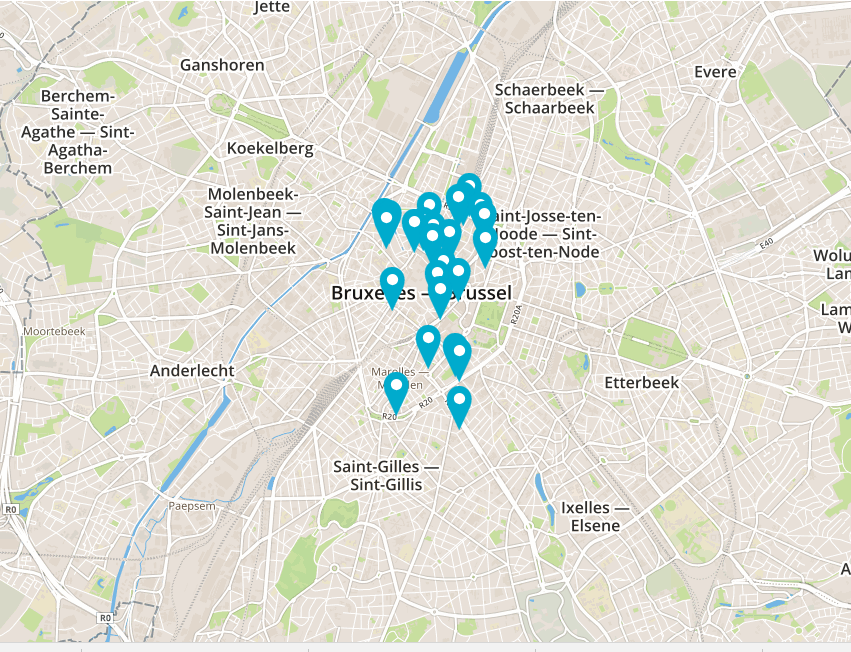
\includegraphics[keepaspectratio=true,width=\textwidth-2cm]{images/publicpark.png}
\end{figure}

The long term private parking has another purpose, to park the car for a long time or every day at the same spot. This parking option is not captured by \bp although having a private parking is not always possible and \bp could thus help the driver to find a place every day.

\subsubsection{Short Term Parking Offers}

Here is a list of selected competitors for \bp .

\begin{itemize}
\item \textbf{Parkopedia} offers to book a parking spot in parking lot online. It allows the user to compare price, check if there is availability and find an offer close to him. They have a strong presence, they have offers in 75 countries and 6308 cities. Although the business proposes a solution to finding a parking spot, the flaws identified in the previous section still holds, expensive, scarce location and time consuming.
\item \textbf{JustPark}, the services offer private parking rent for half an hour to a year and is available in almost all Europe. On average, the cost is less than 50\% of the parking alternative. It emphasis on popular location such as airports and stadiums. Any owner of a parking spot can add the spot to be rented and its availability. When renting a spot, there is a possibility to add a photo, a description and there is a comment system from previous renter. The owner of the parking selects the price per hour, day, week and month. The owner gets 80\% of what the user pays, the other 20\% goes to the application. Although the service could be used in all of Europe, it seems to be only used in the United Kingdom. Indeed, the application is very successful there but when looking for spot in Brussels, there is no parking available. The company was founded is 2006 in London. They raised venture capital from BMW i Ventures\cite{bmwi} and Index Venture.\cite{iven} They finally raised 1 million £ using crowdfunding, they achieved their target in just four days.\cite{crowd}
\item \textbf{ShareMyPark} has basically the same offer as \textit{JustPark} but it is available only in Brussels. The service has been created last year, in January 2016. The offer is quiet weak, with only a hundred available spots in the city.\footnote{Based on a research for a parking time of one hour in April 2017} On top of short term parking, they also offer long term and business parking.
\item \textbf{MyFlexiPark} is another similar service but this time available in all of Belgium. Launched in 2014.
\end{itemize}

There are other similar services as \textit{JustPark} but they are less successful. Thus \textit{JustPark} is the most successful service and \textit{ShareMyPark} and \textit{MyFlexiPark} are the only ones genuinely present in Brussels.\\
As \textit{ShareMyPark} and \textit{MyFlexiPark} have way less success than \textit{JustPark} overall, the market appear to be not captured in Brussels.\\
The \autoref{smp} shows that the offers in Brussels are way less known and followed than \textit{JustPark}, comforting the idea that Brussels' market is open.

\begin{table}[h]
\centering
\caption{Competitors' social media popularity on April 2017}
\label{smp}
\begin{tabular}{l|l|l|l|}
\cline{2-4}
                               & JustPark & ShareMyPark & MyFelxiPark \\ \hline
\multicolumn{1}{|l|}{Twitter}  & 6 811    & 24          & 31          \\ \hline
\multicolumn{1}{|l|}{Facebook} & 19 121   & 780         & 73          \\ \hline
\end{tabular}
\end{table}

Another point is that \textit{JustPark} announces that they have 750 000 users\cite{jpu} and 25 000 spots available\cite{jpd} whereas \textit{ShareMyPark} and \textit{MyFlexiPark} do not make such claims. A potential explanation is that their user base is too low and would refrain people to register, as seeing the service as unsuccessful.



\subsection{Porter’s Five Forces}
The following Porter's Five Forces analysis will focus on the short term private parking industry in Brussels. As this a rising industry the analysis has to be adapted.\\

\begin{itemize}
\item \textbf{Supplier Power} In this industry, the suppliers are the parking spot owner. They play a key role in the success of the business. Indeed, it is not possible to substitute their spot in any way, their offer is scarce. On the other hand, parking spot owner have a direct benefit in offering their parking spot as they would have a direct revenue in a easy and convenient way, almost no involvement from the owner is needed.\\
The owner of a parking spot alone cannot have the same offer as a coordination service such as the one presented, thus there is close to no possibility of forward integration.\\
As the parking owner have a total control, the supplier power is high.
\item \textbf{Buyer Power} The buyers' behaviour depends upon the situation. Indeed, in neighbourhoods where it is easy to find a parking spot, the driver will not be willing to pay for a parking. On the other hand, in denser area, the driver knows that he will struggle to find a spot and potentially lose lot's of time. In those area, it is common for driver to not even look for a parking spot but to go directly in a parking lot, e.g next to a concert venue. Thus the buyer power depends on the context and would be low in dense area but high in other.\\
Overall, it is important to recall that the driver can always choose to look for a another spot and is price sensitive.
\item \textbf{Threat of Entry} Potential entry in the industry is currently relatively high. Indeed, the market in Brussels is not captured yet and thus there is room for entry. However, if a service implements itself correctly, it would set a huge entry barrier as the network effect are very important for the service. To enter, two elements a required, a online platform and a user base. The platform can be built fairly easily but the user base construction is a complicate process.
\item \textbf{Threat of Substitutes} Two types of substitution can happen. Once in the car, the driver can use another means of parking. If there is available spots in the street, he can use them but as seen, in Brussels he would need to pay as well. The driver also can use a parking lot but this is not available everywhere and thus reduces its impact. This type of substitution threat is medium.\\
On the other hand, the motorist can choose to avoid to use his car as a transport mean. Indeed, public transportation, bicycle and walking are other possibilities. In that case, the user would have no use of a parking spot. Although this is a serious threat, the transportation by car stays a very popular choice.
\item \textbf{Industry Rivalry} Finally, the intern competition of the industry is currently low in Brussels. Indeed the service is not well implemented and barely used thus the competition is very weak. The real competition that is currently taking place is the one of the most successful service. As analysed in the threat of entry, if a service succeed to impose itself as the leading one and achieves  having a sufficient user base, then the network effect will make it the winner of the competition.
\end{itemize}

\chapter{Company and Product Description}

\bp will propose to the population of Brussels a fast, cheap and convenient way to park its car in the dense road of the city. Currently, similar online services exist but they struggle to find a user base, a crucial need of the service. Indeed, the success of the offer relies on network effects and once a service hit the critical mass, it will set high entry barrier for other similar services. As opposed to the current offer \bp will place the incentive for parking owner to rent their driveway on the collectivism impact instead of the profit generation.\\

As opposed to the traditional way of parking, \bp will be offering a way for driver to find a place that is :
\begin{itemize}
\item \textbf{Fast}, by using the service, the driver will be guided to a spot. Indeed, a proposition of the nearest available locations will be displayed.
\item \textbf{Cheap}, the price of the parking will be the half of the in street parking.
\item \textbf{Convenient}, it will be possible for the driver to stay long period of time, whereas the in street parking is often limited in time.
\end{itemize} 

Payment will be made online, through debit card and credit card. The renter will be able to withdraw his money from its location made through the service by bank transfer. The renter can also keep the money on its account for his personal use of the service, as a parking spot hunter.\\

As seen in the industry overview, the market target is quite large. Indeed, the service is useful for people who use their car in Brussels. The challenge is to build an offer of parking spot large enough, thus to attract enough parking owner on the service.

\section{Competitive Strategy}
As explained in \autoref{poc}, \bp's offer is matching as demand that is currently not captured by the available parking service.\\

On the other, \bp has to attract the same customer that its competitor are targeting in Brussels. The angle of action is to focus on the collectivism impact of the application instead of the pure profit generation. It means that for someone to rent his driveway, its goal would be to be part of the service because he would like it to be available for him also in other location.\\
This choice comes from two factors. Firstly, because of the apparent fail on focusing only on profit generation, as it seems to be the case for \textit{ShareMyPark} in Brussels. And secondly, because profit generation is hardly possible. Indeed, let's assume that someone is working from 9 am to 5 pm during week days and is willing to lend his parking during that time. Per month, it would lead to a total of 160 hours of potential renting. Let's assume that the parking is rented all the time, at the same price as the in-street parking. In those ideal conditions, the renter would earn an extra 160\euro  per month. Although not negligible, the money generation is not enough for someone to make a living per example. Moreover, as a parking owner, the renter is expected to have a certain level of lifestyle. To conclude, even in unlikely ideal conditions, the potential profit generation is low. But on the other hand, who has not been in a situation of wanting to park his car without obvious offer available ?\\

To fulfil this aim, \bp will have major differentiation in its policy and its use:
\begin{itemize}
\item \textbf{Fixed Price} : the fares for the parking will be fixed. Indeed, in other services, whether it is  the successful \textit{JustPark} or \textit{ShareMyPark}, the renter chooses its price. This way of implementing the service is aligned with their emphasis on profit generation.\\
The fixed price will serve as a selling argument to attract customer. Our business will be able to guaranty that the price is half of in the street alternative.
\item \textbf{Credit Bonus for Renters} : if a user decide to put a driveway for the community, he will get a free credit on its account, which will allow him to rent other spots using the service.
\item \textbf{Automatic Revenue} : if a user place a parking option on \bp, even if it is not booked, he will receive a small amount credit. This credit would not be with-drawable, it can only be used to rent a spot through the offer.
\end{itemize}

The ideal scenario would be that most of the transaction stays within the service, that renter uses their revenue only to rent other parking spot. Ultimately leading to a service where parking owner just exchange their driveways.

\section{Reaching the Customer and Growth}
To reach the customers, three key elements will be used.\\

The first one is classic advertising. As the business is on-demand based, using technology and mobile phone, it seems appropriate to use online advertisement. Moreover, this type of advertisement allows our company to select our audience. The campaign could then focus people living or working in Brussels and owning a car. Social media advertisement is a good option as well because their user base is large, would represent people who are already using mobile phone application and thus more prone to use \bp's app.\\

The second promotion mean will be referring and word-to-mouth. Taking as an example successful campaign from \textit{Take Eat Easy}, \textit{Uber} and \textit{KeyTrade}, the idea is that if a user refer a new one, both of them receive an amount of credit. This lead to two positives effects, first one it incentive the user to refer their friend, thus increasing the user base. Second one is that the new user will be able to try fro free the service, if he likes it he is likely to use again.\\

Thirdly, the last mean is targeted as parking owner. This promotion will be a physical one. The promotion itself will be a small paper aimed at a parking owner, offering them to put their poorly used driveway on the service. The idea is to hire student to go in the streets of Brussels by bike, and to slide the advertisement under the door of the garages that they cross.\\

Finally, as the service is based on collectivism, its popularity could be increased using local platform designed to promote sharing.

\section{Internal Analysis}
The business is not implemented yet but the following describe the aimed resources and capabilities of it.\\

As tangible resources, the software developed will be its core. Although a software is not tangible, it is classified as so here because it is the key component of the business and will be major investment of the business. There will be three declinations of it, a website, an Android application and an iOS application.\\

The intangible asset will be the reputation of the service and its user base. These two elements will have a key impact in the success of the service as it relies on reaching a critical user mass which will lead for the application to be useful. Opposed to the current offer in the Belgian market, \bp will emphasis on the collectivism effect of the service instead of only the potential profit generation for the parking spot owner. This part will be detailed in a following section.\footnote{link}\\

The human resource component will be quite low at the beginning. The equity holder posses management and computer science skills which is sufficient to develop the business technically and strategically. However, maintenance and support will be needed so hiring will happen. Moreover, the promotion of the service will require other short-term hiring which will be described in the marketing plan.\footnote{link}\\

Finally, the capabilities of \bp will be its ease of use and access but mostly its capacity to establish itself as the only service to share parking spots and building user base. The last point rely on the network effect which is the key to succeeding in the industry.

\section{SWOT}

\chapter{Marketing Plan}

\section{Relevant Market}
Brussels is the home of 1 175 173\cite{ciafb} habitants. The number of car registered in Brussels in 2016 is 486 876.\cite{mtvr} Everyday, there is also 350 000 commuters coming to Brussels.\cite{bxcommu}\\
In 2015, in Brussels there was 266 498 garage, parking or roofed spot. Of all those spots, 55 314 were spots linked to a house, thus with an expected driveway.\cite{atpb}
\chapter{Operation and Team}

\chapter{Critical Risks}

\chapter{Financial Plan}


\bibliographystyle{unsrt}
%\bibliographystyle{plain}
\bibliography{./reference/bibliography}


\end{document}
